\begin{OnehalfSpace}

    \noindent\textbf{RELATO DE EXPERIÊNCIA} 

    Como o próprio nome já diz, o Relato de Experiência trata-se de um trabalho no qual o(s) autor(es) irá(ão) compartilhar uma experiência vivenciada, entretanto, essa experiência é sobre, especificamente, referentes a atividades de extensão. Qualquer outra experiência que não seja de uma atividade de extensão não será aceita. Ressalta-se ainda que essa experiência tem que ser significativa não apenas para os autores, mas também para o campo do qual o trabalho se pauta. Dessa forma, é importante que o(s) autor(es) apresentem dados e suas impressões críticas sobre o assunto abordado, sempre trazendo citações estudiosos da área para fundamentar as análises.

    Deve-se apresentar rapidamente o problema, em seguida a metodologia utilizada e por fim, o relato da experiência, de modo impessoal, informando o público-alvo e demais dados que venham mostrar ao leitor a pertinência do relato, destacando possíveis questionamentos, soluções e intervenções.

    Para enriquecer o relato, pode-se inserir no corpo de texto imagens que retratem a vivência. Todos esses elementos devem estar enumerados e identificados, contendo a fonte. Os dados de identificação devem estar acima da figura, em Times New Roman, tamanho 10, centralizado. Caso a fonte seja dos autores, colocar: Fonte Própria como mostram as imagens abaixo.

    \begin{figure}[H]
        \centering
        \caption{Atividade Experimental}
        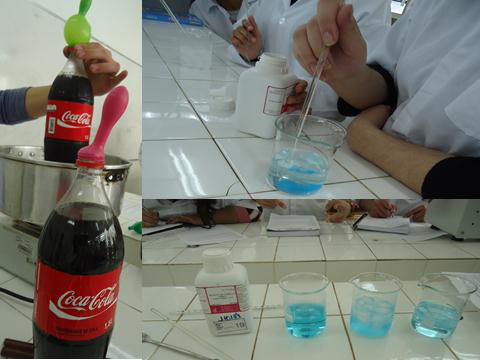
\includegraphics{img/figurateste.png}

        \legend{Fonte: Própria}
        \label{figura}
    \end{figure}

\end{OnehalfSpace}